%This is an Appendix
%%=========================================

\chapter{Source code}
This appendix contains the source code to run the RFEM Plaxis imlementation.
%%=========================================
\section{Introduction}

\lstinputlisting[language=Python, caption=SRM code]{pyt/RFEM01.py}
\lstinputlisting[language=Python, caption=SRM code]{pyt/RFEM02.py}
\lstinputlisting[language=Python, caption=SRM code]{pyt/RFEM03.py}
\lstinputlisting[language=Python, caption=SRM code]{pyt/RFEM04_qc.py}
\lstinputlisting[language=Python, caption=SRM code]{pyt/RFEM05_qc.py}

%%=========================================
\subsection{Starting Python scripting interface - Jupyer notebook}
\begin{figure}[h]
        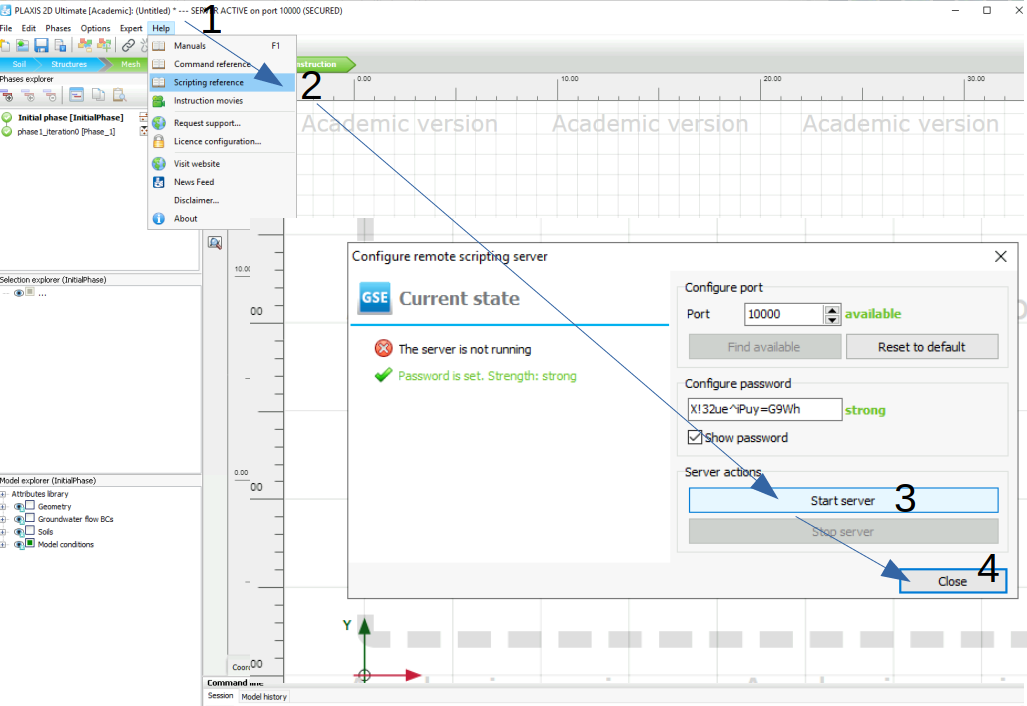
\includegraphics[width=\textwidth]{fig/strt}
	\caption{}
        \label{fig:strtplxs}
\end{figure}

